\documentclass[a4paper, oneside]{book}

\usepackage[utf8]{inputenc}
\usepackage{german}
\usepackage[T1]{fontenc}
\usepackage{a4wide}
\usepackage{listings}
\lstset{
  	literate={ö}{{\"o}}1
           {ä}{{\"a}}1
           {ü}{{\"u}}1
		   {ß}{{\ss}}1,
    % numbers=left,
    showtabs=false,
    breaklines=true,
    showstringspaces=false,
    breakatwhitespace=true,
    basicstyle=\ttfamily,
}

\newcommand{\todo}[1]{
{\color{red}\bf TODO: #1}}
\newcommand{\dg}{DiGaL }

\usepackage{graphicx}

\usepackage[pdfpagelabels]{hyperref}
\hypersetup{
    colorlinks,
    citecolor=black,
    filecolor=black,
    linkcolor=black,
    urlcolor=black
}

\begin{document}
	\begin{titlepage}
		\title{DiGaL}
		\author{Artur Sterz, Jonas Höchst, Andreas Morgen}
		\maketitle
	\end{titlepage}
	\tableofcontents
	\newpage


%!TEX root = report.tex

\chapter{Würfelspiele}
\label{cha:wurfelspiele}

\section{Einführung}
\label{sec:einfuhrung}
	Würfelspiele sind Glücksspiele, die mit Spielsteinen, sogenannten \emph{Würfeln} gespielt werden. Dabei besteht jedes Spiel aus einem oder mehreren Würfeln, die nacheinander oder gleichzeitig geworfen werden, um ein bestimmtes Ergebnis zu erzielen. Hierbei werden von den Spielern kombinatorische Fähigkeiten verlangt.

\section{Wichtige Konzepte}
\label{sec:wichtige_konzepte}
	Für \dg sind im Wesentlichen drei Konstrukte wichtig, die im Nachfolgenden erläutert werden.

	\subsection{Spieler}
	\label{sub:spieler}
		Das erste wichtige Konzept ist der \emph{Spieler}. Den Spieler zeichnet aus, dass er die ausführende Kraft bei einem Spiel ist. Er würfelt mit den Würfeln, bei Entscheidungen muss er diese treffen und auch die Punkteverwaltung hat er inne.

        Weiterhin sind Spielern häufig verschiedene Werte zugeordnet, die zum Beispiel die Punktzahl des Spielers beschreibt. Technisch ausgedrückt lässt sich von Variablen sprechen.

		Und schließlich können Spieler in den meisten Würfelspielen an einem bestimmten Punkt ausscheiden, also vom aktiven in einen inaktiven Zustand übergehen. Beispielsweise kann ein Spieler auf Grund seiner auf 0 reduzierten Punkte aus dem Spiel ausscheiden, er kann aber auch, wie bei dem Spiel \emph{UNO Wüfel} bei einer bestimmten Augenzahl eine Runde aussetzen.

	\subsection{Würfel}
	\label{sub:wurfel}
		Ein weiterer Kernbestandteil sind die Würfel. Dabei kann ein Spiel mehrere Würfel haben, jedoch mindestens einen. Des weiteren hat ein Würfel sogenannte \emph{Augen}. Das bedeutet, dass einer bestimmten Seite ein numerischer Wert zugeordnet wird. Dabei hat ein klassischer Würfel sechs Seiten, ist also von 1 bis 6 durchnummeriert. Es gibt Würfel mit einer ausgefallenen Anzahl an Seiten, aus physikalischen Gründen sind es in der Praxis aber mindestens  zwei Seiten.

		Außerdem sollte noch erwähnt werden, dass es Spiele gibt, bei denen die Würfel keine numerischen Werte besitzen, sondern mit Piktogrammen bedruckt sind. Diese finden in \dg noch keine Anwendung, da sie meistens zu komplexeren Brettspielen gehören und für einfache Spiele eine Repräsentation des Piktogramm durch eine Augenzahl ausreichen sollte.

	\subsection{Spielverlauf}
	\label{sub:spielverlauf}
		Das letzte domänenspezifische Konzept, hier enthalten sein muss, ist der Spielverlauf. Hauptsächlich sind damit die Regeln gemeint, die beschreiben, was ein Spieler zu tun hat, wenn er an der Reihe ist.

		Dabei werden zum einen Aktionen definiert, wie zum Beispiel das Werfen der Würfel. Zum anderen werden aber auch Konditionen geprüft, die erfüllt sein müssen, damit eine Aktion ausgeführt werden kann. So muss beispielsweise bei dem Spiel \emph{Mäxchen} die Augenzahl 21 gewürfelt werden, damit allen anderen Spielern ein Punkt abgezogen werden kann.

\section{Sprachziele}
\label{sec:sprachziele}
	Das oberste Ziel war es \dg so einfach zu gestalten, so dass auch Personen, die keine Programmiererfahrung haben, den vorliegenden Quellcode verstehen können. Die Syntax ist dabei anders als bei herkömmlichen Sprachen und wird hauptsächlich durch Worte ausgedrückt.

	Außerdem wurde versucht die Domäne so genau wie möglich in der Sprache abzubilden. Wie diese Ziele erreicht wurden und welche Kompromisse dabei eingegangen werden mussten, wird in den kommenden Kapiteln ~\ref{cha:die_sprache} und~\ref{cha:designentscheidungen} diskutiert.
%!TEX root = report.tex

\chapter{Die Sprache} % und Designentscheidungen?
\label{cha:die_sprache}
	\section{Grundidee}
	\label{sec:grundidee}
		Bestandteile eines Würfelspiel sind neben den benötigten Materialien wie den Würfeln vor Allem das Regelwerk. Dieses enthält alle Informationen, die benötigt werden, um das Spiel korrekt, also im Sinne des Erfinders, zu spielen. Dabei besteht das Regelwerk aus folgenden Bestandteilen:
		\begin{itemize}
			\item Anzahl der Spieler,
			\item Voraussetzungen für das Spiel,
			\item Aktionen der Spieler,
			\item Spielziel und Bedingungen für das Spielende und,
			\item Bewertungsgrundlagen
		\end{itemize}
		Unser Ziel war es nun \dg so zu gestalten, dass es als Regelwerk eines Spiels erkannt und auch von allen so gelesen werden kann. Damit dies deutlich wird, soll ein Beispiel gegeben werden:
		\subsection{Ein erstes Beispiel}
		\label{sub:ein_erstes_beispiel}
			% TODO: Readable (abstract) syntax or meta-model; Map the syntax elements to domain concepts; ~1000 Wörter
			Um einen ersten Eindruck der Sprache zu erhalten, soll hier zunächst ein Beispielprogramm angegeben werden:\\
\begin{lstlisting}
EINS wird so gespielt:

das spiel ist für 2 bis 10 spieler geeignet.
das spiel hat folgende würfel:
würfel A hat diese seiten: 1 2 3 4 5 6
würfel B hat diese seiten: 1 2 3 4 5 6.

spieler haben die werte PUNKTE ist 0.
spieler haben die werte GEWONNEN ist 0.

ist ein spieler am zug macht er folgendes:
würfelt mit allen würfeln.
rechter spieler ist dran, wenn würfel 0 gleich 1 oder würfel 1 gleich 1.
aktueller spieler PUNKTE ist aktueller spieler PUNKTE + die summe von allen würfeln.
wenn aktueller spieler PUNKTE größergleich 100, dann setze aktueller spieler GEWONNEN auf 1 und spiel ist zu ende.
rechter spieler ist dran.

gewonnen hat der spieler, bei dem GEWONNEN gleich 1.
\end{lstlisting}

	\section{Kontrollierte Sprache}
	\label{sec:kontrollierte_sprache}
		Das oben gezeigte Beispiel, gibt einen ersten Eindruck der Syntax unserer Sprache. 
        Wir haben versucht \dg an die natürlichen Sprache anzulehnen. Es ist unmöglich bzw. ein langer Prozess, alle Eigenheiten der deutschen Sprache zu implementieren und abzubilden. Ein Kompromiss aus unserem Design Goal und der Umsetzbarkeit ist eine kontrollierte Sprache: eine Sprache, die auf der einen Seite zwar intuitiv verständlich ist, auf der anderen Seite jedoch die deutsche Sprache so weit einschränkt, dass sie sinnvoll zu analysieren und grammatisch beschreibbar ist. 
        Das Deklinieren und Konjugieren von Worten ist für das intuitive Verstehen einer Sprache aus unserer Sicht von großer Bedeutung und trägt maßgeblich zum Lesefluss bei. Im obigen Beispiel sei dazu auf auf die Verwendung von \texttt{alle würfel} verwiesen, der im Beispiel schon in seiner deklinierten Variante \texttt{allen würfeln} verwendet wird.
        Auch die Satzstellung ist für das Verständnis einer natürlichen Sprache wichtig. Sätze einer kontrollierten Sprache können schnell sperrig wirken. Unsere Sprache bietet daher verschiedene Optionen um das gleiche auszudrücken. Hier sei als Beispiel das \texttt{wenn} Konstrukt von oben angegeben, dass folgenden beiden Varianten valide ist:
\begin{lstlisting}
rechter spieler ist dran, wenn würfel 0 gleich 1 oder würfel 1 gleich 1.
wenn würfel 0 gleich 1 oder würfel 1 gleich 1, dann rechter spieler ist dran.
\end{lstlisting}
        Designziel der Syntax unserer Sprache ist es zunächst, möglichst viele Varianten eines gegebenen Konstruktes anzubieten, in der Implementierung zeigen sich jedoch Schwierigkeiten, auf die in Kapitel \todo{Ref. einsetzen} näher eingegangen wird.
        
    \section{Satzzeichen} % (fold)
    \label{sec:satzzeichen}
        Wie auch in der natürlichen Sprache, verwenden wir in unserer kontrollierten Sprache Satzzeichen um Mehrdeutigkeit für den Interpretierenden zu verhindern. Die Leser unserer Sprache bestehen nicht nur aus Personen, sondern insbesondere auch vom Parser unserer Implementierung. Die Verwendung von Satzzeichen ist daher obligatorisch.
        \subsection{Punkt (.)} % (fold)
        \label{sub:punkt}
            Punkte schließen Sätze der natürlichen Sprache ab. Unsere kontrollierte Sprache übernimmt dieses Paradigma, um Anweisungen in unserer Sprache abzuschließen. 
        % subsection punkt (end)
        \subsection{Doppelpunkt (:)} % (fold)
        \label{sub:doppelpunkt}
            Der Doppelpunkt leitet Aufzählungen ein. Das erste mal tritt nach dem initialen Satz auf und Leitet die Aufzählung der Definitionsblöcke ein, danach dient er zum Beispiel noch zur Aufzählung er Würfel, deren Seiten, oder der Aktionen, die ein Spieler vollzieht. Der Doppelpunkt dient eher der Übersichtlichkeit als der Eindeutigkeit.
        % subsection doppelpunkt (end)
        \subsection{Komma (,)} % (fold)
        \label{sub:komma}
            Das Komma der natürlichen Sprache trennt Teilsätze ab, die semantisch zusammengehören. In unserer Sprache dienen Kommas dazu mehrere Anweisungen aufzuzählen, und \texttt{dann} und \texttt{sonst} Anweisungen von bedingten Anweisungen abzugrenzen, und die Eindeutigkeit der Programme zu erhalten. 
        % subsection komma (end)
        \subsection{Semikolon (;)} % (fold)
        \label{sub:semikolon}
            Wir verwenden das Semikolon, um den Schleifenrumpf von weiteren folgenden Anweisungen abzutrennen. Dies ist ebenfalls nötig, um die Eindeutigkeit der Sprache zu gewährleisten.
        % subsection semikolon (end)
    % section satzzeichen (end)
    \subsection{Variablen} % (fold)
    \label{sub:variablen}
        Unsere Sprache bietet dem Anwender die domänenspezifischen Objekte \emph{Spieler} und \emph{Würfel}, Variationen davon (\emph{linker/rechter Spieler, Würfel 1, ...}) als Konzept der Sprache an. Darüber hinaus ist es möglich globale Variablen zu definieren, sowie Variablen pro Spieler festzulegen. Spielabhängige Variablen werden in Großbuchstaben geschrieben, um die Trennung von der Syntax zu verdeutlichen (siehe \ref{sec:gross_und_kleinschreibung}).
    % subsection variablen (end)
    \section{Blöcke und Absätze}
    \label{sec:blocke_und_absatze}
     Absätze haben in der natürlichen Sprache den Zweck Abschnitte, die einen eigenen Sinnzusammenhang oder ein eigenes kleines Thema haben von einander abzugrenzen. Dieses Paradigma haben wir auch in der Syntax von \dg übernommen. So haben Programm, die in \dg geschrieben sind vier Absätze, die nach ihrem Sinn unterteilt sind.
 
     Zunächst beginnt ein Programm mit einer Überschrift. Anschließend kommt ein Abschnitt, der die Spielinitialisierung übernimmt. Es werden globale Variablen, Anzahl und Art der Würfel und die Anzahl der Spieler festgelegt. Auch eine Bedingung, wie lange das Spiel läuft, wird hier definiert.
 
     Anschließend folgt ein Abschnitt, in dem die Spieler initialisiert werden, zum Beispiel Spielerspezifische Variablen oder eine Bedingung, wann ein Spieler aktiv ist.
 
     Danach folgt der Abschnitt, in dem die Regeln festgelegt werden, was geschehen soll, wenn ein Spieler an der Reihe ist.
 
     Letztlich gibt es eine Art Schlusssatz, der eine Bedingung definiert, wann ein Spieler gewonnen hat.
 
    \section{Groß- und Kleinschreibung}
    \label{sec:gross_und_kleinschreibung}
     In diesem Punkt weichen wir bewusst von der natürlichen deutschen Sprache ab. Es wäre möglich auch hier die Regeln der deutschen Sprache einzuführen. Das hätte jedoch negative Auswirkungen auf die Lesbarkeit eines Programms. Da \dg eine Programmiersprache ist, bei der es wie bei anderen Programmiersprachen darum geht den Zustand eines Programms zu ändern und das im Wesentlichen über Variablen funktioniert, haben wir uns dazu entschieden Variablenbezeichner komplett groß (z.B. \texttt{EINS} oder \texttt{PUNKTE} in obigem Beispiel) und den Rest komplett klein zu schreiben. Dies erhöht die Lesbarkeit eines Programms und vereinfacht es so Programmierern ein valides und korrektes Programm zu schreiben.
	
    
    \todo{Syntax Tree visualisieren}
%!TEX root = report.tex

\chapter{Designentscheidungen}
\label{cha:designentscheidungen}

\section{Qualitäten der Sprache} % (fold)
\label{sec:qualitaten_der_sprache}


\subsection{Modularität} % (fold)
\label{sub:modularitat}
\subsubsection{Funktionsdefinitionen}
\label{subsub:funktionsdefinitionen}
	\dg bietet keine Konzepte, um Modular Spiele entwickeln zu können. Diese Entscheidung ist bewusst so gewählt worden. Auch hier stand wieder der Fokus im Vordergrund, die Sprache so einfach wie möglich zu gestalten. Ein Programm in Module aufzuteilen heißt zum Beispiel eine Möglichkeit zu bieten Funktionen oder Methoden zu definieren, in denen Aktionen gekapselt sind, die wiederholt ausgeführt werden können. Dies würde aber bedeuten, dass man ein Konzept benötigt, dass einem einen solchen Mechanismus erlaubt. Und dieses neue Konzept müsste von Anwendern unserer Sprache erlernt werden, wenn sie keine Programmierer sind. Daher haben wir uns dazu entschieden, keine Möglichkeit anzubieten Funktionen zu definieren. Es schien uns einfacher dem Nutzer die Möglichkeit zu geben, Aktionen wiederholt zu definieren.

	Desweiteren besteht ein Würfelspiel in \dg aus vier Blöcken, wie sie in \todo{REF EINFÜGEN} vorgestellt werden. Die Möglichkeit Funktionen zu definieren würde daher bedeuten, dass dieses strikte Konzept gebrochen werden müsste, was wiederum ein Mehr an Komplexität bedeuten würde.
\subsubsection{Auslagern in andere Dateien}
\label{subsub:auslagern_in_andere_dateien}
	Da Spiele, die in \dg geschrieben sind, nur aus vier Blöcken bestehen, schien es uns nicht sinnvoll, eine Art der Auslagerung von Code in andere Dateien einzuführen. Auch hier müsste mit dem Konzept der strikten Blockbildung gebrochen werden und eine Möglichkeit geschaffen werden diese Dateien einzubinden oder zu importieren. Das könnte unerfahrene Nutzer jedoch zusätzlich verwirren, da es aus unserer Sicht nicht mit unserem Konzept vereinbar ist, \dg eine kontrollierte Sprache zu Grunde zu legen, da es kein sprachliches Konzept gibt, dass paradigmatisch das gleiche aussagt.

\subsection{Robustheit} % (fold)
\label{sub:robustheit}
Alle \dg Programme haben einen festen Rahmen, dessen freie Flächen durch Variablendefinitionen, Arithmetische Operationen und Kontrollflussanweisungen gefüllt werden. Im Gegensatz zu klassischen Programmiersprachen ist der Programmierer dadurch in seiner Mächtigkeit sehr eingeschränkt. Durch diese Einschränkung ist es ihm wiederum auch weniger leicht möglich, Fehler zu produzieren. Treten Programmierfehler im \dg Programm auf, sind diese schon durch die Syntax invalidiert und können nicht in ein Programm übersetzt werden. Als Beispiel sei hier die Iteration über eine Variable genannt, die in unserer Sprache nur als Iteration über eine Gruppe von Spielern oder Würfeln vorgesehen ist. 

Funktions- oder Klassendefinitionen sind in \dg nicht vorgesehen, der rein Iterative Ansatz reicht aus unserer Sicht aus, den Kontrollfluss und die Komplexität von Würfelspielen zu beschreiben.

Würfelspiele sind in ihren möglichen Ausgängen begrenzt und dadurch gut testbar. Eine kleine Zahl an Würfeln mit seiner geringen Zahl an Würfelflächen, die in einer festen Kontrollstruktur verwendet werden, macht es möglich alle Fälle des Programmes dazu generieren und die Spielausgänge zu testen.
% subsection robustheit (end)

\subsection{Datenmodellierung} % (fold)
\label{sub:datenmodellierung}
\dg bietet keine Möglichkeit um Datenobjekte oder -strukturen anzulegen. Wie unterstützen allerdings einen Aspekt der Objektorientiertheit, in dem wir die Möglichkeit bieten, einem Spieler Variablen zuzuordnen. Die einzigen erweiterterbaren Objekte sind also die Spieler. Alle vom Nutzer definierten Variablen, die nicht zu Spielern gehören lassen sich nur global als Variable des Spiels anlegen.

Als weiteres (nicht modifizierbares) Objekt sind Würfel zu nennen, deren Namen und Seiten zwar vom Programmierer definiert, nicht aber neue Felder hinzugefügt werden können.
% subsection datenmodellierung (end)

\subsection{Abstraktionsniveau} % (fold)
\label{sub:abstraktionsniveau}
	Das Abstraktionsniveau in \dg ist bewusst sehr hoch gewählt. Auch hier stand wieder die Einfachheit der Sprache im Vordergrund. Daher haben wir keinerlei Möglichkeiten geschaffen beispielsweise auf Adressen im Arbeitsspeicher zuzugreifen oder Operationen auf Bits oder Bytes auszuführen. Auch typische Probleme in anderen Programmiersprachen wie Initialisierung oder Speicherverwaltung werden vom Compiler übernommen, sodass sich vor Allem unerfahrene Nutzer nicht um derlei Probleme kümmern müssen. 
% subsection abstraktionsniveau (end)

\subsection{Verständlichkeit} % (fold)
\label{sub:verstandlichkeit}
	Die Verständlichkeit von \dg ist gegeben durch die Verwendung der kontrollierten Sprache. Dadurch ergeben sich keine syntaktisch kryptischen Konstruktionen, die bei späterem Betrachten aufwendig rekonstruiert werden müssen. Auch die Unterstützung von alternativen Formulierungen (siehe \todo{REF}) vereinfacht die Verständlichkeit. Falls sich doch komplexe Ausdrücke ergeben sollten, die nicht auf Anhieb verständlich sind, haben wir die Möglichkeit geschaffen den Code durch Kommentare zu erklären.

% subsection verstandlichkeit (end)
% section qualitaten_der_sprache (end)

\section{Alternativen im Sprachdesign} % (fold)
\label{sec:alternativen_im_sprachdesign} 

Grundpfeiler unserer Sprache ist, maximal einfache Beschreibungen der Domänspezifischen Anwendungen auszudrücken, in Anlehnung an die natürliche Sprache. Würden wir auf diese Eigenschaft verzichten, wäre die Begründung für die Einschränkungen nicht mehr gegeben und alle oben genannten Punkte müssten neu diskutiert werden, da die Begründung sich weitestgehend auf das erste Argument stützt. 

Zur Problemlösung wäre auch eine Library denkbar, die Paradigmen aus Würfelspielen aufgreift und dem Nutzer zur einfacheren Implementierung anbietet. Durch die sehr auf die Domäne ausgerichtete Sprache, folgen die meisten oben diskutierten Entscheidungen direkt. Einzelne Paradigmen lassen sich jedoch diskutieren und in Frage stellen.

\subsection{Erweiterung bestehender Spiele}
\label{sub:erweiterung_bestehender_spiele}
	Eine weitere Möglichkeit der Modularisierung ist bestehende Spiele, also in unserem Fall bestehenden Code zu erweitern. Die aktuell \dg Version bietet dieses Konstrukt nicht an. Denkbar wäre aber eine Art Vererbung, in dem ein Spiel auf einem anderen Basiert und jeder Block um weitere Anweisungen ergänzt werden kann (hinzufügen von Würfeln, zusätzliche Aktionen bei bestimmten Ergebnissen, ...). Diese Vererbung sollte ein Spiel jedoch nur erweitern, nicht aber bestehende Regeln außer Kraft setzen können, da dies zum einen wieder zu Lasten der Verständlichkeit geschehen würde. Zum andern würde eine Änderung des zugrundeliegenden Spieles faktisch einer Neuentwicklung gleich kommen und sollte aus diesem Grund auch so behandelt werden.
% section modularitat (end)

\subsection{Mächtigkeit} % (fold)
\label{sub:machtigkeit}
Um die Ausdrucksmächtigkeit von \dg zu erhöhen ist eine wesentliche Änderung Funktionen einzuführen. Der Programmierer könnte Konstrukte definieren, die im Moment von der Sprache zur Verfügung gestellt werden und damit den Code besser strukturieren. 

Eine weitere Möglichkeit um die Ausdrucksmächtigkeit zu erhöhen liegt darin, frei zu definierende \emph{while} Schleifen einzuführen. Im Moment werden in der Sprache lediglich \emph{foreach} und \emph{for} Schleifen angeboten. Die bereits eingeführten Konstrukte zur Iteration könnten verallgemeinert werden, so dass auch Variablen definiert werden können, über die iteriert werden kann. Dies würde allerdings zu Lasten der Robustheit gehen, da der Programmierer dadurch leichter Fehler machen kann, die erst zur Laufzeit auftreten.
% subsection machtigkeit (end)

\subsection{Objektmodellierung} % (fold)
\label{sub:objektmodellierung}
Einige Spiele bestehen nicht nur aus den von uns unterstützten Datenstrukturen \emph{Spieler} und \emph{Würfel}. So hat beispielsweise das Spiel Kniffel neben genannten Objekten auch noch Spielzettel mit Ergebniswerten und Becher. Diese können zwar in \dg mit Spielervariablen nachgebildet werden, eine Modellierung als Objekt wäre jedoch auch denkbar und unter Umständen wünschenswert.

Außerdem gibt es in manchen Spielen Spieler, die eine Sonderrolle haben und von uns auch nicht direkt unterstützt werden. Auch hier würde eine Möglichkeit der Modellierung sinnvoll sein.

Schließlich existieren Spiele, die Objekte aus anderen Domänen übernehmen, Zum Bespiel Spielkarten oder Spielfelder und Spielfiguren, die sich auf den Spielfeldern bewegen.\\

Um diese Dinge zu unterstützen könnte das Konzept der Objektorientiertheit eingeführt werden und damit einhergehen auch Möglichkeiten um eigenen Objekte zu erstellen und zu modellieren.

% subsection objektmodellierung (end)
% section alternativen_im_sprachdesign (end)

\section{Designspace} % (fold)
\label{sec:designspace}

\subsection{Werte \& Typen} % (fold)
\label{sub:werte_typen}
Unsere Domäne erfordert keine ausgefallenen Datentypen. Würfelseiten und daraus resultierend auch die Aktionen im Spiel basieren auf Ganzzahl-Werten \emph{(Integer)}. Variablen in unserer Sprache werden mit Strings adressiert, die aus Großbuchstaben bestehen. Der Datentyp String besteht in der Sprache selbst nicht und wird bei der Kompilation im Endprodukt hinzugefügt. Denkbar wäre es allerdings, Strings einzuführen, zum Beispiel um eigene textuelle Ausgaben zu definieren, die vom gegebenen Framework abweichen.

Darüber hinaus werden die domänenspezifischen Objekte direkt adressiert. Für Spieler gibt es Ausdrücke, die den jeweils linken oder rechten Spieler des aktuellen oder einen Spieler auf einem bestimmten Platz adressieren. Ebenso ist es möglich Würfel über deren Nummer oder Bezeichnung zu adressieren. Mengen von Würfeln oder Spieler können über deren verschiedene Eigenschaften ausgewählt werden: \emph{alle}, \emph{aktive (spieler)}, \emph{würfel 1, würfel 2}.
% subsection werte_typen (end)

\subsection{Dispatching} % (fold)
\label{sub:dispatching}
	Dispatching beschreibt den Umstand, dass bei polymorphen Methoden zur Laufzeit entschieden werden muss, welche Methode ausgeführt wird: die der eigenen Klasse oder die der Superklasse. Da \dg weder Methoden noch Vererbung unterstützt, mussten wir uns keine Gedanken zu Dispatching machen.

% subsection dispatching (end)

\subsection{Ausdrücke} % (fold)
\label{sub:ausdrucke}
	\dg unterstützt alle gängigen arithmetischen Ausdrücke außer die Division, da bei Würfelspielen in den meisten Fällen nur mit ganzzahlen gerechnet wird. Außerdem würde die Division einen neuen Datentypen für Fließkommazahlen voraussetzen, den wir aber der Einfachheit halber nicht unterstützen.
	
	Außerdem sind Vergleichsoperationen wie \texttt{größer}, \texttt{kleiner}, \texttt{gleich} möglich. Auch logische Ausdrücke wie \texttt{und} und \texttt{oder} sind möglich.
	
	Weiterhin gibt es domänenspezifische Ausdrücke. Hier sei die Operatione \texttt{die summe von} genannt, die die summe aller gewürfelten Augenzahlen ermittelt und die Operation \texttt{anzahl}, die die Anzahl von zum Beispiel aktiven Spielern zurück gibt.

% subsection ausdrucke (end)

\subsection{Scope} % (fold)
\label{sub:scope}
	Bei einem Würfelspiel sind zu Beginn alle Variablen global bekannt. Wenn gewürfelt wird, sehen alle Spieler die gewürfelte Augenzahl und auch alle Spieler wissen, wie viele Spieler und Würfel am Spiel beteiligt sind. Daher gibt es im Spiel lediglich einen globalen Scope. In diesem können auch alle Spieler alle Werte lesen und verändern.
	
	Die Spieler hingegen haben eigene lokale Variablen, da diese nicht zum globalen Spiel gehören, sondern jeder Spieler für beispielsweise seine eigenen Punkte verantwortlich ist. Es gibt jedoch die Möglichkeit Werte von anderen Spielern zu ändern. Dies ist bewusst so entschieden worden, da beispielsweise bei dem Spiel Mäxchen bei der Augenzahl 21 allen anderen Spielern ein Punkt abgezogen wird.

% subsection scope (end)

\subsection{Anweisungen} % (fold)
\label{sub:anweisungen}
DiGaL bietet dem Nutzer eine eingeschränkte, aber sehr domänenspezifische Sammlung an Anweisungen. Elementare Anweisungen sind Zuweisungen (von ausgewerteten Ausdrücken), Schleifen und bedingte Anweisungen, die so auch in klassischen Programmiersprachen auftreten.

Darüber hinaus sind die Elementaren Ausdrücke unserer Domäne als feste Anweisungen vorgesehen: \emph{würfeln mit }, \emph{sortieren}, \emph{nächster spieler ist dran}, ... Diese festen Anweisungen können als eine Art Framework für Würfelspiele aufgefasst werden.


% subsection anweisungen (end)

% section designspace (end)





%!TEX root = report.tex

\chapter{Prototyp Implementierung}
\label{cha:implementierung}

In der Referenzimplementierung von \dg verwenden wir die ANTLR Syntax zur formalen Definition unserer Sprache. Darauf aufbauen verwenden wir den von ANTLR bereitgestellten Parser und Lexer zum das in \dg geschriebene Spiel zu erfassen. \\

    \begin{figure}[ht]
    	\centering
        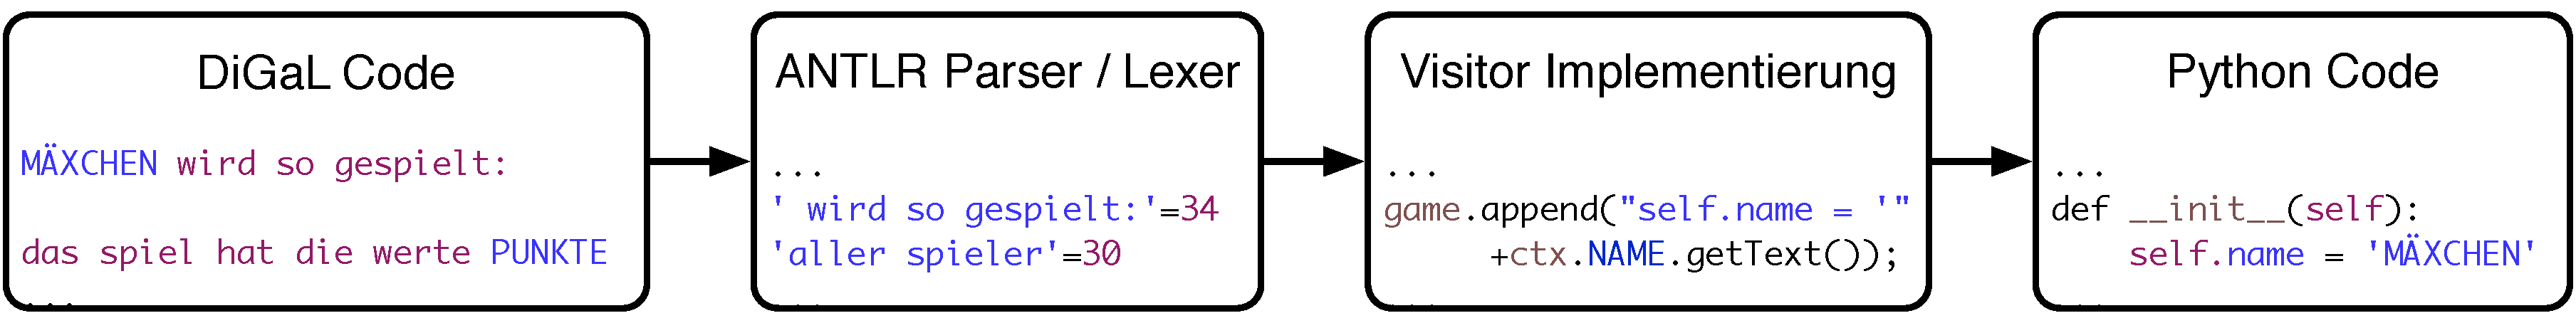
\includegraphics[width=\textwidth]{Flow.pdf}
    	\caption{Ablauf der Kompilation eines DiGaL Programmes}
    	\label{flow}
    \end{figure}

Um sicherzustellen, dass die mit \dg geschriebenen Spiele portabel sind, haben wir uns zum Ziel gesetzt möglichst wenige Abhängigkeiten vorauszusetzen. 
Ein Kriterium war dabei, dass die Ausführung des Codes nur mit der Standardbibliothek einer Zielsprache funktioniert. Wir haben uns deswegen für eine Kompilation der Sprache entschieden, und verzichten für den Endanwender auf die Installation von ANTLR. Als Zielsprache wählten wir Python, das Syntaktisch kompakt zu programmieren ist und inhärente Konzepte unserer Sprache unterstützt (Objektorientiertheit, Funktionale Programmierung). 

Zur Generierung des Python Codes haben wir uns für das Visitorpattern entschieden. Die Entscheidung gründet auf die Simplizität einer Implementierung dieses Patterns, das uns als lernende ANTLR Spielentwickler nur noch abverlangt die vorgegebenen Methoden zu implementieren und uns so auf das wesentlich zu konzentrieren. 

\section{Python Framework} % (fold)
\label{sec:python_framework}
    
    Zusammen mit der Definition der Grammatik haben wir generische Methoden ausgearbeitet. Die vorhanden Methoden lassen sich in zwei Klassen differenzieren: Generische Methoden, die in vielen Würfelspielen verwendet werden; Methoden die zur Interaktion mit den Mitspielern und zur Repräsentation von Daten gegenüber diesen nötig sind. Die zweite Gruppe ergibt sich nicht aus der Domäne selbst, sondern folgt aus der nötigen Mensch-Maschine Kommunikation (Ausgaben auf der Kommandozeile).
    
    \begin{figure}[ht]
    	\centering
        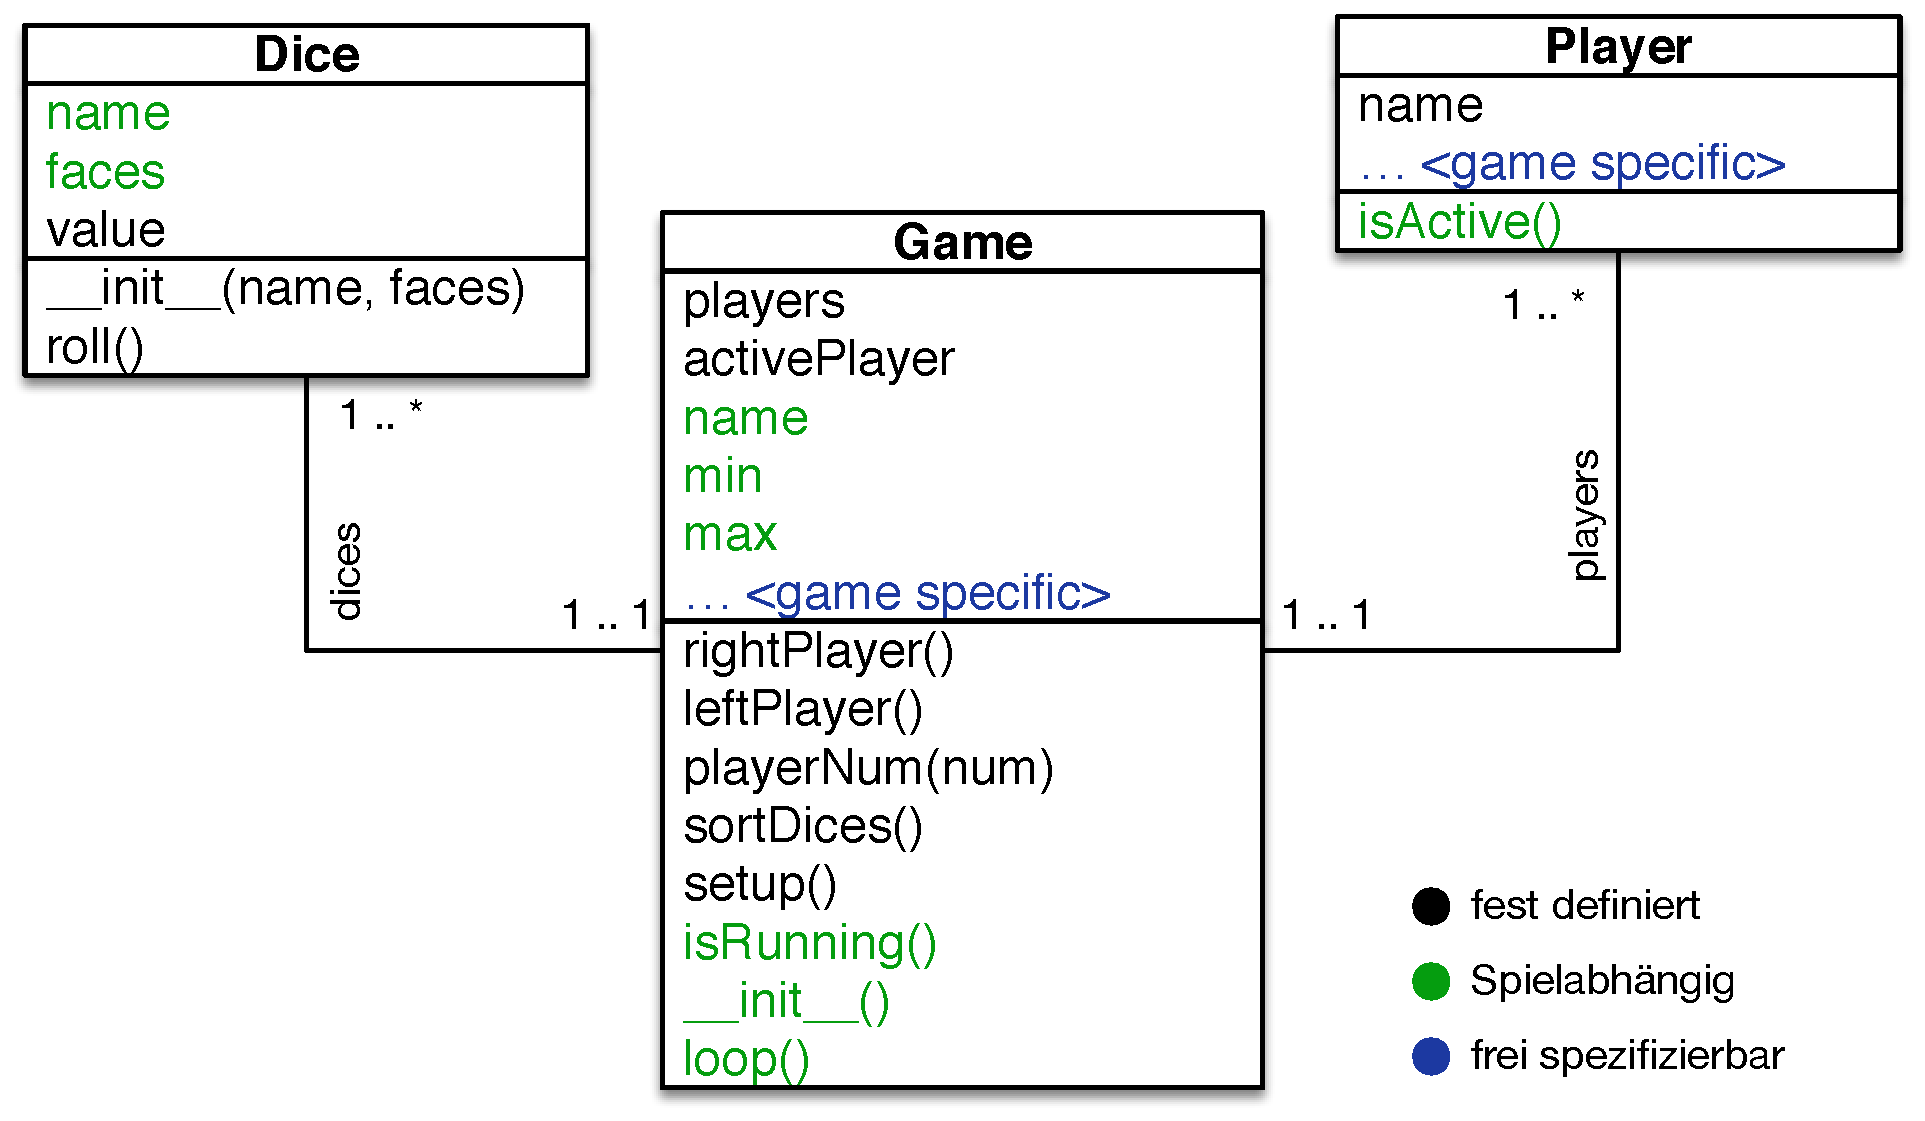
\includegraphics[width=0.8\textwidth]{Python-UML.pdf}
    	\caption{Klassendesign des Python Frameworks}
    	\label{python-uml}
    \end{figure}
    
    Die Domänenspezifischen Methoden können direkt aus der Sprache verwendet werden und entsprechen den verwendbaren Anweisungen (\texttt{würfelt mit <würfeln>}).
    
\section{Interne Datenrepräsentation} % (fold)
\label{sec:interne_datenreprasentation}
    Wie in den oben Abschnitten erwähnt, verwenden wir für die Implementierung Konstrukte unserer Zielsprache. Der objektorientierte Ansatz von \dg zeigt sich hier in der Umsetzung in Klassen für Spieler, Würfel und das Spiel selbst. Bei der Übersetzung eines Spiels werden Teile der gegebenen Klassen durch die vom Spielentwickler spezifizierten Eigenschaften des Spiels ergänzt. Beispiel dafür sind die Spieler, denen durch den Spielentwickler neuen Felder hinzugefügt werden können.Die Würfelklasse hingegen ist nicht erweiterbar, sondern wird nur durch die Implementierung der Spielklassen verschieden initialisiert.
    
    Die Spielklasse enthält die Initialisierung und den Ablauf des Spiels und ist die zentrale Klasse. Die Klasse enthält einige generische Methoden, die nicht individualisierbar sind und in der Sprache zur Verfügung stehen (\texttt{leftPlayer()}, \texttt{rightPlayer()}, \texttt{sortDices()}, ...). In Kontrast dazu bildet die \texttt{loop()}-Methode den Spielablauf ab und wird vom Entwickler frei definiert.
% section interne_datenreprasentation (end)
    
% section python_framework (end)

\section{Compilerimplementierungen}
\label{sec:compilerimplementierungen}
	Da die Implementierung recht umfangreich ist kann sie hier nicht vollständig angegeben werden. Daher beschränken wir uns hier auf einige Beispiele.
	
\dg wurde so konzipiert, dass alle Domänenspezifischen Konzepte, wie sie oben beschrieben sind, direkt abgebildet werden können. Auch in der Pythonumsetzung haben wir versucht dies beizubehalten, und die Konzepte von \dg soweit wie möglich direkt in Python umzusetzen. Grundoperationen wie \texttt{+, -, *, größer, kleiner, gleich, ...} haben wir direkt in ihren entsprechenden Pythonoperatoren umgesetzt, woraus eine lazy evaluation arithmetischer Operationen folgt. Gleiches gilt für die Zuweisung. Diese kann in \dg zwar syntaktisch unterschiedlich ausgedrückt werden (\texttt{<Variable> ist <Ausdruck>} oder \texttt{setze <Variable> auf <Ausdruck>}), in Python wird daraus aber immer eine einfache Zuweisung.
	
		Des weiteren haben wir einige Abstraktionen vorgenommen, um die Paradigmen aus der Domäne umzusetzen. Als Beispiel sei folgender Code gegeben:
\begin{lstlisting}
wenn würfel A gleich 2 ...
\end{lstlisting}
		In konventionellen Programmiersprachen wäre diese Operation nicht ohne weiteres möglich, da ein Vergleich zwischen einem selbst definierten Objekt und einer Zahl zunächst nicht definiert ist. Im Bezug auf die Domäne ist dieser Ausdruck jedoch sinnvoll, da damit implizit gemeint ist, dass der gewürfelte Wert, also eine Zahl mit einer anderen verglichen werden soll. Diesen Umstand nutzen wir, sodass ein logischer Vergleich oder eine arithmetische Operation mit Würfeln immer als Operation auf dem entsprechenden gewürfelten Wert zu verstehen ist. Im Code sieht das wie folgt aus:

\begin{lstlisting}
if [dice for dice in self.dices if dice.name == 'A'].value == 2 ...
\end{lstlisting}
Diese Idee haben wir versucht so weit wie möglich umzusetzen. Sie findet sich beispielsweise in der Referenzierung des nächsten Spielers wieder. Hier genügt es in \dg zum Beispiel das Schlüsselwort \texttt{linker spieler} zu verwenden. Diese Abstraktion haben wir in Python so umgesetzt, dass der Index der Liste, in dem Spieler gespeichert sind, um ein dekrementiert wird.

Weiterhin soll hier auf die Implementierung der Methode \texttt{isRunning()} eingegangen werden. Diese repräsentiert die Bedingung, die der Entwickler festlegen kann. Sie bestimmt, ob ein Spiel noch läuft oder nicht. Beispielsweise kann ein Spiel nach $n$ Runden zu Ende sein.

\begin{lstlisting}[label={lst:ODD}]
ODD wird so gespielt:

das spiel hat den wert RUNDEN ist 5.
...
das spiel läuft solange RUNDEN größer 0.
...
\end{lstlisting}
	Im oberen Listing wird beispielsweise die globale Variable \texttt{RUNDEN} definiert und als Bedingung festgelegt, dass ein Spiel solange läuft, solange \texttt{RUNDEN größer 5} gilt. Das heißt das Spiel läuft fünf Runden. Im kompilierten Pythoncode sieht das wie folgt aus:
\begin{lstlisting}[language=Python]
def isRunning(self): return (self.RUNDEN > 0)
\end{lstlisting}
Diese Methode hat eine weitere Besonderheit. Wird keine Bedingung festgelegt, weil ein Spiel beispielsweise kein deterministisches Ende hat, sondern von Fall zu Fall unterschiedlich ist, hat die Funktion einen Standardfall, bei dem immer \texttt{true} zurückgegeben wird. In diesem Fall muss sich der Entwickler aber selbst darum kümmern, das Spiel mit den Schlüsselwort \texttt{das spiel ist zu ende.} zu beenden. Methoden dieser Art, also die gegeben sein müssen, aber vom Nutzer gefüllt werden können, gibt es noch weitere, beispielsweise die Funktion \texttt{isActive()}, die nach einer von Entwickler definierten Bedingung entscheidet, ob ein Spieler aktiv ist oder nicht.


\section{Erfüllung der geforderten Sprachqualitäten} % (fold)
\label{sec:erfullung_der_geforderten_sprachqualitaten}
Zentrale Qualität der Sprache ist die Einfachheit und die daraus folgende Robustheit durch Einschränkung der Mächtigkeit. Ein Beispiel für die Erfüllung dieses Kriteriums liegt in der automatischen Interpretation von Würfelreferenzen. Wird ein Würfel in einer arithmetischen Operation verwendet, so wird stets der aktuell angezeigte Wert referenziert. Dem Spieleentwickler ist es damit nicht möglich einen Würfel mit einer Zahl zu addieren, er adressiert in diesem Fall automatisch das Ergebnis.

Ein Beispiel, dem die geforderte Robustheit noch fehlt ist die Verwendung von \texttt{für}-Schleifen. Der Nutzer muss hier einen Bezeichner definieren, auf den er im Schleifenrumpf zugreifen kann. Denkbar wäre eine vereinfachte Version, in der Variablen des iterierten Objektes und die des globalen Scopes zusammenliegen und direkt verwendet werden können. Diese Variante würde die Syntax vereinfachen, wir haben uns in dieser Version unserer Sprache zu gunsten einer einfacheren Implementierung für eine konventionelle For-Schleife entschieden.
% section erfullung_der_geforderten_sprachqualitaten (end)

\section{Mögliche Erweiterungen} % (fold)
\label{sec:mogliche_erweiterungen}
	Im laufe der Entwicklung von \dg haben wir Konzepte entwickelt und diskutiert, die es nicht in die Implementierung geschafft haben oder sich im Nachhinein als falsch oder unzulänglich erwiesen haben.
	
	Zunächst wäre da die Implementierung des Frameworks zu nennen. Hier gibt es in der aktuellen Version konkrete Klassen, die dynamisch mit den von Nutzer spezifizierten Elementen gefüllt werden. Da wir mit Python jedoch eine Objektorientierte Sprache verwenden, wäre es sinnvoller abstrakte Basisklassen von Spieler, Würfeln und dem Spiel zur Verfügung zu stellen, von denen eine implementierte Klasse angelegt wird, die von der entsprechenden Klasse erbt. Somit hätte man auch die Objektorientiertheit, die in \dg teilweise inhärent gegeben ist auch auf die Implementierung angewandt. Eine Möglichkeit der Modularität wäre somit gegeben, die uns in der aktuellen Version jedoch verloren geht.
	
	Außerdem hat \dg einige syntaktische Konstrukte, die von unserer Entscheidung, die Sprache so intuitiv und einfach wie möglich zu gestalten abweichen. Zu erwähnen ist die Adressierung und Referenzierung von Würfeln. Im aktuellen Zustand haben Würfel Namen, die der Entwickler vorgeben muss. Will man nun den Wert dieses Würfels haben, kann das auf zwei Arten geschehen. Entweder über den Namen oder über einen Index. Dieser Index wird allerdings erst logisch sinnvoll, wenn eine sortierung der Würfel stattgefunden hat. Und die Adressierung über den Namen scheint nicht aus der Domäne hervorzugehen, da man Würfeln normalerweise keine Namen gibt. Um das zu erleichtern oder intuitiver zu gestalten, könnten beispielsweise neue syntatkische Konstrukte wie \emph{Pasch} oder \emph{Straße} eingeführt werden, die die Überprüfung dieser Ereignisse vereinfacht.
	
	Schließlich waren zu Beginn Konstrukte geplant, die es dem Entwickler ermöglichen eigene Nutzerinteraktion zu definieren, beispielsweise Ausgaben auf der Kommandozeile oder die Möglichkeit auf Ereignisse dynamisch zu reagieren und nicht nur nach fest definierten Regeln vorzugehen. Unser Fokus lag jedoch zunächst auf den Konzepten, die von der Domäne gegeben sind und die Sprache möglichst einfach zu gestalten. Daher wurde dieser Punkt mit einer niedrigen Priorität hinten angestellt und ist in der aktuellen Referenzimplementierung nicht enthalten.
    

% section mogliche_erweiterungen (end)













%!TEX root = report.tex

\chapter{Erfahrungen}
\label{cha:erfahrungen}

Die erste Lektion, die wir gelernt haben, ist, dass das Konzept der natürlichen Sprache Mehrdeutigkeiten mitbringen. Um diese Mehrdeutigkeiten zu verhindern, müssten wir Konstrukte wie Klammern oder erweiterte Interpunktion einführen, was jedoch mit diesem Konzept brechen würde. Als folge der Verwendung natürlicher Sprache wurde das gleichzeitige Erlernen und Implementieren der Sprache mit Hilfe von ANTLR zu einer Herausforderung, sodass viel Zeit auf diesen Teil verwendet werden musste und einige diskutierten Konzepte nicht umgesetzt werden konnten. Auch für die Implementierung konnte nur ein kleiner Anteil der Zeit investiert werden. Als Lehre daraus ziehen wir, dass wir in künftigen Neuentwicklungen auf eine formellere, aber dennoch leicht zu verstehende Sprache setzen würden. Statt nur auf die Sprache zu setzen, wäre es denkbar den Entwickler durch eine einfache, Baukastenartige Entwicklungsumgebung zu unterstützen.

Weiterhin haben wir versucht, möglichst viele Konzepte, die die Domäne mitbringt, in \dg umzusetzen. Im Laufe der Entwicklung haben wir festgestellt, dass eine strikte Umsetzung dieser Konzepte Nachteile mit sich bringt. Für Fortgeschrittene Nutzer sind weitergehende Konzepte, die nicht domäneninhärent sind wünschenswert. Hier ist an erste Stelle das Konzept der Vererbung im Sinne der Erweiterbarkeit von Spielen zu nennen.


Außerdem würden wir zunächst die benötigten Technologien lernen, sodass sich die Konzeption der Sprache und die Erlernung dieser nicht gegenseitig behindern. Auch eine iterative Entwicklung, bei der zunächst kleine Teile implementiert und diese anschließend erweitert werden ist wünschenswert. Die Wahl der zugrundeliegenden Technologien wie beispielsweise Parsergeneratoren sollte fundiert getroffen und ausführlich diskutiert werden, da verschiedene Technologien zu unterschiedlichen Zwecken entwickelt wurden.

Schließlich haben wir in der Umsetzung des Compilers einige Konzepte von \dg nicht direkt übernommen, was uns an manchen Punkten Schwierigkeiten bereitet hat, da bereits erdachte und diskutierte Lösungen umgeworfen werden mussten. Beispielsweise gibt es in \dg nur einen globalen Scope, der in Python jedoch unzulänglich umgesetzt ist. Auch eine bessere Wahl der Zielsprache könnte diskutiert werden. Es sollte eine Sprache gewählt werden, die der eigenen konzeptuell möglichst nah ist. In einer Neuimplementierung würden wir auf Java setzen, um das Framework als Sammlung von abstrakten Superklassen umzusetzen und die Spiele davon erben zu lassen. Eine Erweitarbarkeit von Spielen wäre ebenfalls einfach implementierbar. Denkbar wäre auch eine Implementierung, die nicht als Compiler sondern als Interpreter umgesetzt ist.
    
    \newpage



	

\end{document}
